\documentclass[10pt,aspectratio=169]{beamer}

\usetheme{metropolis}
\usepackage{appendixnumberbeamer}

\usepackage{booktabs}
\usepackage{tabularx}
\usepackage{multirow}
\usepackage{colortbl}
\usepackage{graphicx}
\usepackage{tikz}
\usepackage{pgfplots}
\pgfplotsset{compat=1.16}
\usetikzlibrary{shapes,arrows,positioning}

\usepackage{amsmath}
\usepackage{amssymb}

% Colors
\definecolor{winnergreen}{RGB}{39, 174, 96}
\definecolor{warningorange}{RGB}{230, 126, 34}
\definecolor{errorred}{RGB}{192, 57, 43}

\title{RRMC: Robust Revision-MI Control}
\subtitle{Stopping Rule Evaluation on AR-Bench Detective Cases}
\date{\today}
\author{RRMC Team}
\institute{Active Reasoning Benchmark Experiments}

\begin{document}

\maketitle

\begin{frame}{Table of Contents}
  \setbeamertemplate{section in toc}[sections numbered]
  \tableofcontents[hideallsubsections]
\end{frame}

%==============================================================================
\section{Background: Stopping Methods}
%==============================================================================

\begin{frame}{The Active Reasoning Problem}
  \begin{block}{Goal}
    When should an LLM \textbf{stop asking questions} and provide a final answer?
  \end{block}
  
  \vspace{0.5cm}
  
  \textbf{AR-Bench Detective Cases (DC):}
  \begin{itemize}
    \item LLM plays detective, asks yes/no questions to an oracle
    \item Must identify the correct suspect from candidates
    \item Trade-off: More questions $\rightarrow$ more information but higher cost
  \end{itemize}
  
  \vspace{0.5cm}
  
  \textbf{Key Metrics:}
  \begin{itemize}
    \item \textbf{Accuracy}: Correct suspect identification rate
    \item \textbf{Avg Turns}: Average questions asked before stopping
  \end{itemize}
\end{frame}

\begin{frame}{Method Overview: Simple Baselines}
  \begin{columns}[T]
    \begin{column}{0.48\textwidth}
      \textbf{Fixed Turns}
      \begin{itemize}
        \item Always ask exactly $N$ questions
        \item No adaptive stopping
        \item Baseline comparison
      \end{itemize}
      
      \vspace{0.5cm}
      
      \textbf{Verbalized Confidence}
      \begin{itemize}
        \item Ask LLM: ``Rate confidence 1-10''
        \item Stop when confidence $\geq$ threshold
        \item Simple but relies on self-assessment
      \end{itemize}
    \end{column}
    
    \begin{column}{0.48\textwidth}
      \textbf{Self-Consistency}
      \begin{itemize}
        \item Sample $k$ answers at temperature $>0$
        \item Stop when majority agrees ($\geq$ threshold)
        \item Measures answer stability
      \end{itemize}
      
      \vspace{0.5cm}
      
      \textbf{Semantic Entropy}
      \begin{itemize}
        \item Cluster semantically similar answers
        \item Compute entropy over clusters
        \item Stop when entropy $<$ threshold
      \end{itemize}
    \end{column}
  \end{columns}
\end{frame}

\begin{frame}{Method Overview: MI-Based Methods}
  \begin{columns}[T]
    \begin{column}{0.48\textwidth}
      \textbf{MI-Only}
      \begin{itemize}
        \item Estimate Mutual Information via self-revision
        \item $\text{MI} = H[\text{answers}] - H[\text{answers}|\text{revision}]$
        \item Stop when MI $<$ threshold
        \item Low MI = new info won't change answer
      \end{itemize}
      
      \vspace{0.3cm}
      
      \textbf{Robust MI}
      \begin{itemize}
        \item Multi-variant MI estimation
        \item Uses ``base'' and ``skeptical'' prompts
        \item More robust uncertainty quantification
      \end{itemize}
    \end{column}
    
    \begin{column}{0.48\textwidth}
      \textbf{Key Insight}
      \begin{alertblock}{MI Interpretation}
        \textbf{High MI}: Model uncertain, new questions likely to change answer
        
        \textbf{Low MI}: Model confident, safe to stop
      \end{alertblock}
      
      \vspace{0.3cm}
      
      \textbf{Threshold Effect}
      \begin{itemize}
        \item Lower threshold $\rightarrow$ stricter stopping criterion
        \item Requires more certainty before stopping
        \item Results in more turns but higher accuracy
      \end{itemize}
    \end{column}
  \end{columns}
\end{frame}

\begin{frame}{Method Overview: New Baselines}
  \begin{columns}[T]
    \begin{column}{0.48\textwidth}
      \textbf{KnowNo}
      \begin{itemize}
        \item Conformal prediction approach
        \item Build prediction sets with coverage guarantees
        \item Stop when set size $\leq$ threshold
        \item From: Ren et al. (2023)
      \end{itemize}
      
      \vspace{0.3cm}
      
      \textbf{CIP-Lite}
      \begin{itemize}
        \item Simplified conformal inference
        \item Track answer set across samples
        \item Stop when answers converge
      \end{itemize}
    \end{column}
    
    \begin{column}{0.48\textwidth}
      \textbf{UoT-Lite}
      \begin{itemize}
        \item Inspired by Uncertainty of Thoughts
        \item Lightweight variant for stopping
        \item Uses answer diversity as signal
      \end{itemize}
      
      \vspace{0.5cm}
      
      \begin{block}{Implementation Status}
        These methods are newly ported from literature. Grid search reveals they may stop too early on DC tasks.
      \end{block}
    \end{column}
  \end{columns}
\end{frame}

%==============================================================================
\section{Initial Method Runs}
%==============================================================================

\begin{frame}{Initial Baseline Results (5 puzzles)}
  \begin{table}
    \centering
    \begin{tabular}{lccc}
      \toprule
      \textbf{Method} & \textbf{Threshold} & \textbf{Accuracy} & \textbf{Avg Turns} \\
      \midrule
      Fixed Turns (5) & -- & 40\% & 5.0 \\
      Self-Consistency & 0.7 & 20\% & 1.0 \\
      Semantic Entropy & 0.5 & 20\% & 1.0 \\
      Verbalized Confidence & 8.0 & 20\% & 1.0 \\
      MI-Only & 0.3 & 20\% & 1.0 \\
      Robust MI & 0.3 & 20\% & 1.0 \\
      \bottomrule
    \end{tabular}
  \end{table}
  
  \vspace{0.3cm}
  
  \begin{alertblock}{Problem Identified}
    Most methods stop at \textbf{Turn 1} with only 20\% accuracy!
    
    $\rightarrow$ Thresholds too permissive, triggering immediate stops
  \end{alertblock}
\end{frame}

%==============================================================================
\section{Parameter Grid Search}
%==============================================================================

\begin{frame}{Grid Search Methodology}
  \begin{block}{Objective}
    Find optimal thresholds for each stopping method
  \end{block}
  
  \vspace{0.3cm}
  
  \textbf{Setup:}
  \begin{itemize}
    \item 5 puzzles per threshold value (quick iteration)
    \item Parallel execution across 6 terminals
    \item Track accuracy and average turns
  \end{itemize}
  
  \vspace{0.3cm}
  
  \textbf{Threshold Ranges Tested:}
  \begin{table}
    \centering
    \small
    \begin{tabular}{ll}
      \toprule
      \textbf{Method} & \textbf{Values Tested} \\
      \midrule
      MI-Only & 0.01, 0.02, 0.05, 0.1, 0.2, 0.3 \\
      Robust MI & 0.01, 0.02, 0.05, 0.1, 0.2, 0.3 \\
      Verbalized Confidence & 5.0, 6.0, 7.0, 8.0, 9.0 \\
      Self-Consistency & 0.5, 0.6, 0.7, 0.8, 0.9, 1.0 \\
      Semantic Entropy & 0.05, 0.1, 0.2, 0.3, 0.5 \\
      \bottomrule
    \end{tabular}
  \end{table}
\end{frame}

\begin{frame}{Grid Search Results}
  \begin{table}
    \centering
    \begin{tabular}{lcccc}
      \toprule
      \textbf{Method} & \textbf{Best Threshold} & \textbf{Accuracy} & \textbf{Avg Turns} & \textbf{Note} \\
      \midrule
      \rowcolor{winnergreen!20}
      \textbf{MI-Only} & \textbf{0.01} & \textbf{80\%} & \textbf{6.0} & $\star$ Winner \\
      Verbalized Conf. & 9.0 & 80\% & 20.6 & Expensive \\
      \midrule
      Semantic Entropy & 0.5 & 40\% & 1.0 & Stops early \\
      Self-Consistency & 1.0 & 40\% & 1.6 & Stops early \\
      KnowNo & 2--3 & 40\% & 1.0 & Stops early \\
      CIP-Lite & 1 & 40\% & 1.6 & Stops early \\
      \bottomrule
    \end{tabular}
  \end{table}
  
  \vspace{0.3cm}
  
  \begin{columns}[T]
    \begin{column}{0.48\textwidth}
      \begin{exampleblock}{Key Finding}
        \textbf{MI-Only with threshold=0.01} achieves 80\% accuracy with only 6 turns average.
      \end{exampleblock}
    \end{column}
    \begin{column}{0.48\textwidth}
      \begin{alertblock}{Issue}
        Methods stopping at Turn 1 are just guessing without gathering information.
      \end{alertblock}
    \end{column}
  \end{columns}
\end{frame}

\begin{frame}{MI-Only: Threshold vs Performance}
  \begin{center}
  \begin{tikzpicture}
    \begin{axis}[
      width=0.8\textwidth,
      height=0.6\textheight,
      xlabel={MI Threshold},
      ylabel={Accuracy (\%)},
      xmin=0, xmax=0.35,
      ymin=0, ymax=100,
      xtick={0.01, 0.05, 0.1, 0.2, 0.3},
      ytick={0, 20, 40, 60, 80, 100},
      legend pos=north east,
      grid=major,
      nodes near coords,
      every node near coord/.append style={font=\small, anchor=south},
    ]
    \addplot[
      color=blue,
      mark=*,
      thick,
      point meta=explicit symbolic,
    ] coordinates {
      (0.01, 80) [80\%]
      (0.05, 60) [60\%]
      (0.1, 40) [40\%]
      (0.2, 20) [20\%]
      (0.3, 20) [20\%]
    };
    \end{axis}
  \end{tikzpicture}
  \end{center}
  
  \textbf{Insight}: Lower threshold $\rightarrow$ stricter stopping $\rightarrow$ more turns $\rightarrow$ higher accuracy
\end{frame}

%==============================================================================
\section{Validation Results \& Analysis}
%==============================================================================

\begin{frame}{Validation Results: The Early-Stopping Problem}
  \begin{alertblock}{Grid Search Did NOT Generalize!}
    Results on 20 puzzles reveal a fundamental problem.
  \end{alertblock}
  
  \vspace{0.2cm}
  
  \begin{table}
    \centering
    \small
    \begin{tabular}{lcccc}
      \toprule
      \textbf{Method} & \textbf{Accuracy} & \textbf{Avg Turns} & \textbf{Turn 1 \%} & \textbf{MI=0 \%} \\
      \midrule
      CIP-Lite & 45\% & 1.4 & 75\% & -- \\
      KnowNo & 40\% & 1.0 & \textcolor{errorred}{\textbf{100\%}} & -- \\
      Self-Consistency & 35\% & 1.1 & 90\% & 75\% \\
      Semantic Entropy & 35\% & 1.4 & 80\% & 75\% \\
      Fixed Turns (10) & 30\% & 10.0 & 0\% & -- \\
      Verbalized Conf. & 30\% & 23.1 & 0\% & -- \\
      \rowcolor{errorred!20}
      MI-Only (0.01) & \textbf{25\%} & 4.1 & 70\% & \textbf{70\%} \\
      Robust MI & 25\% & 3.0 & 70\% & 45\% \\
      \bottomrule
    \end{tabular}
  \end{table}
  
  \textbf{Grid search showed 80\% for MI-Only, but validation shows only 25\%!}
\end{frame}

\begin{frame}{Root Cause: MI = 0 at Turn 1}
  \begin{columns}[T]
    \begin{column}{0.55\textwidth}
      \textbf{MI Scores for MI-Only (first 10 puzzles):}
      \begin{table}
        \centering
        \small
        \begin{tabular}{ccc}
          \toprule
          \textbf{Puzzle} & \textbf{MI at Turn 1} & \textbf{Result} \\
          \midrule
          0--4 & \textcolor{errorred}{\textbf{0.0}} & Stop $\rightarrow$ Wrong \\
          5 & 0.45 & 4 turns $\rightarrow$ Wrong \\
          6--7 & \textcolor{errorred}{\textbf{0.0}} & Stop $\rightarrow$ Mixed \\
          8 & 0.45 & 5 turns $\rightarrow$ Wrong \\
          9 & \textcolor{errorred}{\textbf{0.0}} & Stop $\rightarrow$ Correct \\
          \bottomrule
        \end{tabular}
      \end{table}
    \end{column}
    
    \begin{column}{0.42\textwidth}
      \begin{alertblock}{The Problem}
        At Turn 1, LLM generates \textbf{identical answers} across all k=6 samples.
        
        \vspace{0.2cm}
        
        Identical $\rightarrow$ zero entropy $\rightarrow$ \textbf{MI = 0}
        
        \vspace{0.2cm}
        
        MI = 0 $<$ 0.01 $\rightarrow$ \textbf{Immediate stop}
      \end{alertblock}
    \end{column}
  \end{columns}
  
  \vspace{0.3cm}
  
  \begin{block}{Fundamental Issue}
    MI estimator conflates ``model is confident'' with ``model has enough information.''
    
    At Turn 1 with \textbf{zero clues gathered}, a confident model is just \textbf{guessing}.
  \end{block}
\end{frame}

\begin{frame}{Analysis: Why Grid Search Misled Us}
  \begin{columns}[T]
    \begin{column}{0.48\textwidth}
      \textbf{Grid Search (5 puzzles):}
      \begin{itemize}
        \item 80\% accuracy, 7.4 avg turns
        \item Those 5 puzzles happened to have \textbf{diverse initial samples}
        \item Non-zero MI triggered more turns
        \item \textcolor{warningorange}{\textbf{Lucky variance!}}
      \end{itemize}
    \end{column}
    
    \begin{column}{0.48\textwidth}
      \textbf{Validation (20 puzzles):}
      \begin{itemize}
        \item 25\% accuracy, 4.1 avg turns
        \item 70\% of puzzles: MI = 0 at start
        \item 70\% stopped at Turn 1
        \item True performance revealed
      \end{itemize}
    \end{column}
  \end{columns}
  
  \vspace{0.5cm}
  
  \begin{alertblock}{Key Lesson}
    \textbf{5 puzzles is not enough} for reliable threshold tuning.
    
    Small sample variance can create misleading ``winners.''
  \end{alertblock}
\end{frame}

\begin{frame}{Turn Distribution Analysis}
  \begin{columns}[T]
    \begin{column}{0.48\textwidth}
      \textbf{MI-Only Turn Distribution:}
      \begin{table}
        \centering
        \small
        \begin{tabular}{ccc}
          \toprule
          \textbf{Turns} & \textbf{Count} & \textbf{Accuracy} \\
          \midrule
          1 & 14 & 28.6\% \\
          4--5 & 2 & 0\% \\
          8 & 1 & 100\% \\
          12--14 & 2 & 0\% \\
          25 (max) & 1 & 0\% \\
          \bottomrule
        \end{tabular}
      \end{table}
    \end{column}
    
    \begin{column}{0.48\textwidth}
      \textbf{Verbalized Confidence:}
      \begin{table}
        \centering
        \small
        \begin{tabular}{ccc}
          \toprule
          \textbf{Turns} & \textbf{Count} & \textbf{Accuracy} \\
          \midrule
          2--9 & 2 & 0\% \\
          25 (max) & 18 & 33.3\% \\
          \bottomrule
        \end{tabular}
      \end{table}
      
      \vspace{0.3cm}
      
      \textit{Opposite problem: never stops, always hits max turns!}
    \end{column}
  \end{columns}
  
  \vspace{0.3cm}
  
  \textbf{Observation:} Methods either stop too early (Turn 1) or too late (Turn 25). No method finds the sweet spot.
\end{frame}

\begin{frame}[fragile]{Concrete Example: Turn-1 Stop (No Questions Asked)}
  \begin{columns}[T]
    \begin{column}{0.48\textwidth}
      \textbf{Puzzle 0 - WRONG}
      \begin{itemize}
        \item Prediction: Suspect 0
        \item Ground Truth: Suspect 3
        \item MI at Turn 1: \textbf{0.0}
        \item Questions asked: \textbf{NONE}
      \end{itemize}
      
      \vspace{0.3cm}
      
      \texttt{Conversation: []}
      
      \vspace{0.3cm}
      
      \textit{Model guessed without asking a single question!}
    \end{column}
    
    \begin{column}{0.48\textwidth}
      \textbf{Puzzle 1 - CORRECT (lucky)}
      \begin{itemize}
        \item Prediction: Suspect 0
        \item Ground Truth: Suspect 0
        \item MI at Turn 1: \textbf{0.0}
        \item Questions asked: \textbf{NONE}
      \end{itemize}
      
      \vspace{0.3cm}
      
      \texttt{Conversation: []}
      
      \vspace{0.3cm}
      
      \textit{Same behavior -- just happened to guess correctly.}
    \end{column}
  \end{columns}
  
  \vspace{0.3cm}
  
  \begin{alertblock}{14/20 puzzles stopped at Turn 1 with empty conversations!}
    The model is ``confidently guessing'' -- all k=6 samples agree on same answer before asking anything.
  \end{alertblock}
\end{frame}

\begin{frame}[fragile]{Concrete Example: Multi-Turn Success (Rare)}
  \textbf{Puzzle 17 - CORRECT after 8 turns}
  
  \vspace{0.2cm}
  
  \small
  MI Scores: [0.22, 0.64, 0.78, 0.41, 0.87, 0.64, 1.01, \textbf{0.0}]
  
  \vspace{0.2cm}
  
  \begin{tabular}{cl}
    Turn 1: & Asked Eleanor Whitaker: ``What were you doing near the studio?'' \\
    Turn 2: & Asked Michael Turner: ``Who was with you at the project site?'' \\
    Turn 3: & Asked Clara Mitchell: ``Did you have disagreements with Jonathan?'' \\
    ... & \\
    Turn 8: & MI drops to 0.0 $\rightarrow$ Stop $\rightarrow$ \textcolor{winnergreen}{\textbf{Correct!}} \\
  \end{tabular}
  
  \vspace{0.3cm}
  
  \begin{exampleblock}{What went right}
    \begin{itemize}
      \item Model was uncertain from start (MI = 0.22 > 0)
      \item Asked diverse questions to different suspects
      \item Gradually gathered information until confident
      \item \textbf{Only 1 of 6 multi-turn puzzles succeeded (16.7\%)}
    \end{itemize}
  \end{exampleblock}
\end{frame}

\begin{frame}[fragile]{Concrete Example: Multi-Turn Failure (Common)}
  \textbf{Puzzle 18 - WRONG after 25 turns (max)}
  
  \vspace{0.2cm}
  
  \small
  Prediction: Suspect 0 | Ground Truth: Suspect 2
  
  MI never stabilized: [0.32, 0.26, 1.24, 0.87, ... , 0.87, $\infty$]
  
  \vspace{0.2cm}
  
  \begin{tabular}{cl}
    Turn 1: & Asked Clara Bennett: ``What were you doing 9-10pm?'' \\
    Turn 2: & Asked Marcus Langley: ``Did you have disputes with Jonathan?'' \\
    Turn 3: & Asked Dr. Harper: ``Were you in the office 9-10pm?'' \\
    ... & \\
    \textcolor{errorred}{Turn 22:} & \textcolor{errorred}{Asked Marcus Langley: \textbf{SAME QUESTION}} \\
    \textcolor{errorred}{Turn 23:} & \textcolor{errorred}{Asked Dr. Harper: \textbf{SAME QUESTION}} \\
    Turn 25: & Hit max turns $\rightarrow$ \textcolor{errorred}{\textbf{Wrong!}} \\
  \end{tabular}
  
  \vspace{0.2cm}
  
  \begin{alertblock}{Problems identified}
    \begin{itemize}
      \item Model asks \textbf{repetitive questions} (same suspect, same question)
      \item Doesn't synthesize information across turns
      \item MI never drops $\rightarrow$ runs to max turns $\rightarrow$ still wrong
    \end{itemize}
  \end{alertblock}
\end{frame}

%==============================================================================
\section{Conclusions \& Proposed Fixes}
%==============================================================================

\begin{frame}{Key Takeaways}
  \begin{enumerate}
    \item \textbf{All current stopping methods fail on DC task}
    \begin{itemize}
      \item Best accuracy: 45\% (CIP-Lite) -- barely better than random
      \item MI-Only dropped from 80\% (5 puzzles) to 25\% (20 puzzles)
    \end{itemize}
    
    \vspace{0.3cm}
    
    \item \textbf{The MI = 0 problem is fundamental}
    \begin{itemize}
      \item At Turn 1, LLM samples are often identical $\rightarrow$ MI = 0
      \item Zero MI triggers immediate stop before gathering information
      \item 70--100\% of puzzles stop at Turn 1 for most methods
    \end{itemize}
    
    \vspace{0.3cm}
    
    \item \textbf{Grid search on small samples is unreliable}
    \begin{itemize}
      \item 5 puzzles showed 80\% accuracy (lucky variance)
      \item 20 puzzles revealed true 25\% performance
      \item Need larger validation sets (50+) for reliable tuning
    \end{itemize}
  \end{enumerate}
\end{frame}

\begin{frame}{Proposed Fixes}
  \begin{columns}[T]
    \begin{column}{0.48\textwidth}
      \textbf{1. Minimum Turns Guard}
      \begin{itemize}
        \item Force at least $N$ turns before checking MI
        \item E.g., \texttt{min\_turns = 3}
        \item Ensures some information gathering
      \end{itemize}
      
      \vspace{0.3cm}
      
      \textbf{2. MI Floor with Context}
      \begin{itemize}
        \item Only stop if MI $<$ threshold \textbf{AND} turns $>$ min
        \item Combine uncertainty with effort
      \end{itemize}
    \end{column}
    
    \begin{column}{0.48\textwidth}
      \textbf{3. Diversity Detection}
      \begin{itemize}
        \item Detect when samples are identical
        \item If all same $\rightarrow$ don't trust MI = 0
        \item Force temperature increase or more sampling
      \end{itemize}
      
      \vspace{0.3cm}
      
      \textbf{4. Progressive Threshold}
      \begin{itemize}
        \item Start with high threshold (keep asking)
        \item Gradually lower as turns increase
        \item Natural ``explore then exploit''
      \end{itemize}
    \end{column}
  \end{columns}
\end{frame}

\begin{frame}{Next Steps}
  \begin{itemize}
    \item \textbf{Implement minimum turns guard}: Quick fix to prevent Turn-1 stops
    \item \textbf{Larger validation}: Run on 50+ puzzles for reliable metrics
    \item \textbf{Analyze sample diversity}: Understand when/why samples collapse
    \item \textbf{Cross-task evaluation}: Test on Situation Puzzles (SP), Guessing Numbers (GN)
    \item \textbf{Calibration pipeline}: Use risk-controlled threshold calibration with larger calibration set
  \end{itemize}
  
  \vspace{0.5cm}
  
  \begin{center}
    \large\textbf{Thank you!}
    
    \vspace{0.3cm}
    
    \normalsize Code: \texttt{github.com/[repo]/RRMC}
  \end{center}
\end{frame}

\end{document}
